\section{Strong-baseline anchors, scaling and assumption controls}
\label{app:post-supplementary}

The supplementary allowance contains 1,600 anchor logs and 100 negative-control
logs, separate from the primary E1--E5 grids. All methods and both confidence
levels share each complete log. The server environment was selected by an
explicit amendment before the first outcome in either supplementary suite;
the unused original local freezes are preserved. No already-started primary
suite changed production environment. All 1,718 returned artifact files were
verified against their server byte hashes; this file count is not a trial count.

\subsection{Theorem-compatible strong comparisons}

The homogeneous IID anchor has $N=32768$, one coordinate, logging probabilities
$(.75,.25)$, target $(.5,.5)$, nuisance .5, target mean .45 and threshold .4.
The finite-moment Catoni comparator receives the legal centered-moment bound
proved in Appendix~\ref{app:post-iid-anchor}; it is not given an unproved generic
conversion from a raw residual moment. The scalar betting comparator is the
authors' one-dimensional implementation, not the full two-dimensional MOPE
procedure. DR empirical Bernstein is applied under its independent-data
filtration contract. None of these anchor results licenses an arbitrary
graph-dependent application of an IID theorem.

All 68 eligible primary anchor cell--method comparisons have complete-family
coverage in 200/200 trials, no observed false claim and no Holm undercoverage
flag. The marginal Wilson 95\% coverage interval for each fixed comparison is
$[.981155,1]$. Table~\ref{tab:post-iid} shows that the stronger independent
comparators can be narrower. One scalar-betting interval misses the target at
the secondary 90\% level, giving 199/200 coverage there and 200/200 at the
primary 95\% level. That checkpoint is retained as
\texttt{COMPLETE\_WITH\_CONFIDENCE\_FAILURE}. The runner counts it as one failed
unit, while the analysis reports zero execution failures. These are different
fields, not different retained samples.

\begin{table}[tbp]
\centering
\small
\begin{tabular}{lrrrr}
\toprule
 & \multicolumn{2}{c}{IID bounded} & \multicolumn{2}{c}{IID finite moment}\\
Method & Width & Detected & Width & Detected\\
\midrule
COMET / matched generic & .01748 & 200/200 & .17416 & 0/200\\
Graph Bernstein & .01748 & 200/200 & NA & NA\\
Catoni & .02740 & 200/200 & .15246 & 0/200\\
Scalar OPE betting & .01941 & 200/200 & NA & NA\\
Independent DR EB & .01055 & 200/200 & NA & NA\\
\bottomrule
\end{tabular}
\caption{Eligible strong anchors at the primary 95\% level. Width is the mean
intersected interval width, in the original target scale. Detected means a true
violation certified in a complete trial. All displayed eligible methods cover
200/200 targets. Missing entries are theorem-ineligible, rather than zero
performance. Full method and secondary-level rows remain in the exports.}
\label{tab:post-iid}
\end{table}

\subsection{Fixed-DGP scaling}

The connected-cycle anchors use 16 coordinates and $N$ in
$\{8192,32768,131072\}$, with 200 independent complete logs in each
sample-size/outcome cell. COMET's mean intersected coordinate widths are
$.03424,.01666,.00821$ in the bounded model and
$.19071,.12153,.07664$ in the finite-moment model. Every applicable method
detects a violation in 200/200 bounded logs and 0/200 finite-moment logs at
each size. Coverage is 200/200 throughout at the primary level.
The width averages retain the fixed auditor family, whose coordinates have
different known feasible ranges. Their decline is descriptive evidence for
this design sequence, not validation of a minimax rate, a necessary sample
size, or useful detection in the tested finite-moment regime.

\subsection{Incorrect premises and omitted bias}

Four prespecified controls have 25 complete logs each and threshold .6.
Their mechanisms are specified in the preceding proof appendix. Deliberately
invalid intervals retain their heuristic label and never inherit a
certificate guarantee. Under wrong propensities, evaluation-nuisance leakage
and omission of clipping bias, these intervals make false-safe claims in
25/25 trials. Under a hidden shared shock they make false-violation claims in
13/25 trials. All four heuristic arms have 0/25 interval coverage.
The 13/25 false-claim frequency has marginal Wilson 95\% interval
$[.334985,.699687]$; the 25/25 and 0/25 endpoints are
$[.866808,1]$ and $[0,.133192]$ respectively.

Correctly specified reference intervals cover 25/25 targets in each control.
The exact-exposure and independent-nuisance references detect their true
violations in 25/25 trials. In contrast, the shared-shock known-range reference
and bias-debited clipping certificate have width one and detect none.
Vacuous coverage is retained as such. Truthfully disclosed unsupported
requests are refused in 25/25 trials per control; their coverage and error
rates are not applicable. Refusal is not evidence that a schema can discover
an undisclosed shock, incorrect exposure law or nuisance leakage from one log.

\begin{figure}[tbp]
\centering
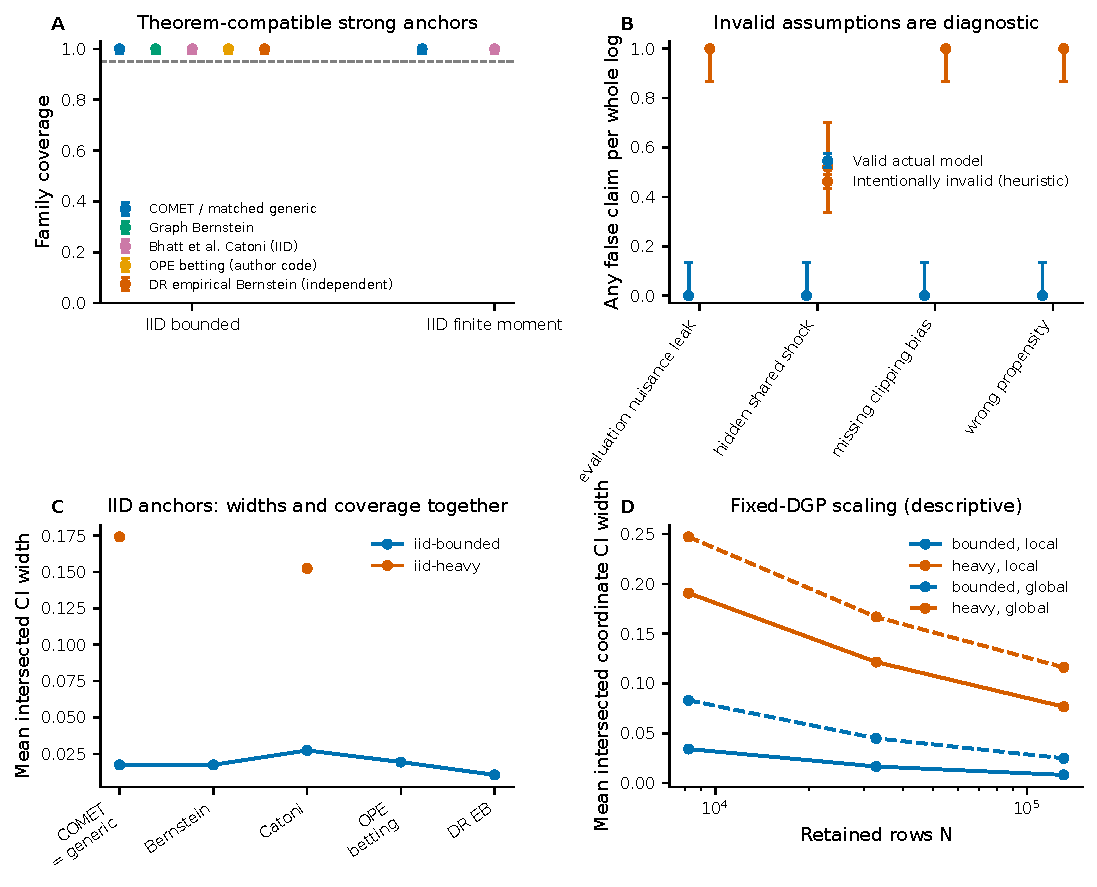
\includegraphics[width=\linewidth]{figures/supplementary_server_v2_v1/appendix_anchors_controls.pdf}
\caption{Supplementary evidence. Anchor coverage and negative-control false
claims have pointwise whole-log Wilson 95\% intervals. Widths are intersected
interval widths, not empirical moment estimates. The independent/bounded
comparators appear only where eligible; honest refusals have no error rate
and are omitted from that panel. Every fixed cell and both levels remain in
the accompanying exports, including the secondary betting coverage miss.}
\label{fig:post-supplementary}
\end{figure}
